\documentclass[12pt,letterpaper]{article}\usepackage[]{graphicx}\usepackage[]{color}
%% maxwidth is the original width if it is less than linewidth
%% otherwise use linewidth (to make sure the graphics do not exceed the margin)
\makeatletter
\def\maxwidth{ %
  \ifdim\Gin@nat@width>\linewidth
    \linewidth
  \else
    \Gin@nat@width
  \fi
}
\makeatother

\definecolor{fgcolor}{rgb}{0.345, 0.345, 0.345}
\newcommand{\hlnum}[1]{\textcolor[rgb]{0.686,0.059,0.569}{#1}}%
\newcommand{\hlstr}[1]{\textcolor[rgb]{0.192,0.494,0.8}{#1}}%
\newcommand{\hlcom}[1]{\textcolor[rgb]{0.678,0.584,0.686}{\textit{#1}}}%
\newcommand{\hlopt}[1]{\textcolor[rgb]{0,0,0}{#1}}%
\newcommand{\hlstd}[1]{\textcolor[rgb]{0.345,0.345,0.345}{#1}}%
\newcommand{\hlkwa}[1]{\textcolor[rgb]{0.161,0.373,0.58}{\textbf{#1}}}%
\newcommand{\hlkwb}[1]{\textcolor[rgb]{0.69,0.353,0.396}{#1}}%
\newcommand{\hlkwc}[1]{\textcolor[rgb]{0.333,0.667,0.333}{#1}}%
\newcommand{\hlkwd}[1]{\textcolor[rgb]{0.737,0.353,0.396}{\textbf{#1}}}%

\usepackage{framed}
\makeatletter
\newenvironment{kframe}{%
 \def\at@end@of@kframe{}%
 \ifinner\ifhmode%
  \def\at@end@of@kframe{\end{minipage}}%
  \begin{minipage}{\columnwidth}%
 \fi\fi%
 \def\FrameCommand##1{\hskip\@totalleftmargin \hskip-\fboxsep
 \colorbox{shadecolor}{##1}\hskip-\fboxsep
     % There is no \\@totalrightmargin, so:
     \hskip-\linewidth \hskip-\@totalleftmargin \hskip\columnwidth}%
 \MakeFramed {\advance\hsize-\width
   \@totalleftmargin\z@ \linewidth\hsize
   \@setminipage}}%
 {\par\unskip\endMakeFramed%
 \at@end@of@kframe}
\makeatother

\definecolor{shadecolor}{rgb}{.97, .97, .97}
\definecolor{messagecolor}{rgb}{0, 0, 0}
\definecolor{warningcolor}{rgb}{1, 0, 1}
\definecolor{errorcolor}{rgb}{1, 0, 0}
\newenvironment{knitrout}{}{} % an empty environment to be redefined in TeX

\usepackage{alltt}
\usepackage[utf8]{inputenc}
\usepackage[margin=.7in]{geometry}
\usepackage{graphicx}
\usepackage{titling}
\usepackage{amsmath}
\usepackage{amsfonts}
\usepackage{amssymb}
\renewcommand{\theenumiv}{\arabic{enumiv}}
\setlength{\droptitle}{-5em}
\author{Maurice Diesendruck\vspace{-2ex}}
\title{StatMod2 - Hierarchical Models and Shrinkage - Polls\vspace{-1ex}}
\IfFileExists{upquote.sty}{\usepackage{upquote}}{}
\begin{document}
\maketitle

\section{Summary}
Albert and Chib (1993) present exact Bayesian methods for posterior sampling
of binary response data. Where a probit regression would normally be used,
they augment the model by introducing a left- or right-truncated normal
variable Z, that corresponds to 1- or 0-valued y response, respectively. 
In doing so, the model enables standard linear model results for normal-normal
posteriors, which can be used to find full conditionals for Gibbs sampling.

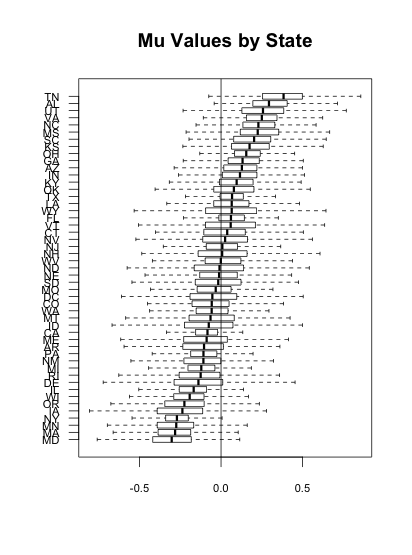
\includegraphics[height=13cm, keepaspectratio]{polls-mus.png}
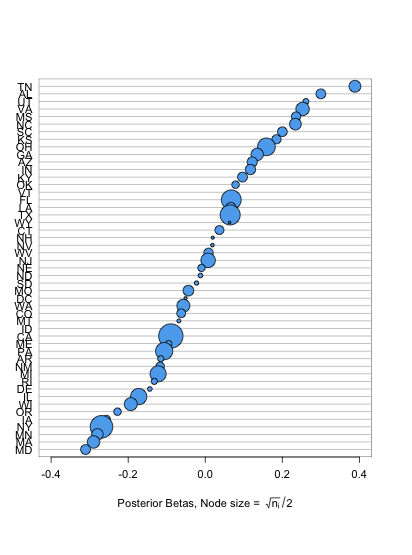
\includegraphics[height=13cm, keepaspectratio]{polls-posterior-mus.png}\\
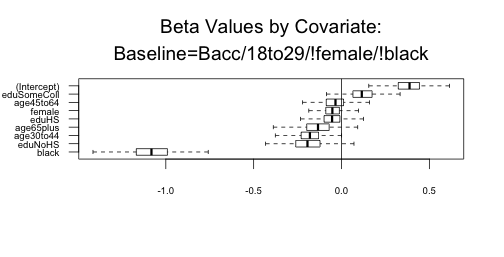
\includegraphics[height=5cm, keepaspectratio]{polls-betas.png}
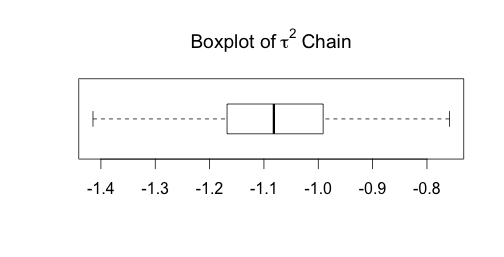
\includegraphics[height=5cm, keepaspectratio]{polls-tausq.png}\\

\section{Full R Code}
\begin{knitrout}
\definecolor{shadecolor}{rgb}{0.969, 0.969, 0.969}\color{fgcolor}\begin{kframe}
\begin{alltt}
\hlcom{# StatMod2 - Polls}

\hlkwd{library}\hlstd{(MASS)}
\hlkwd{library}\hlstd{(truncnorm)}
\hlkwd{library}\hlstd{(Hmisc)}

\hlcom{#####}
\hlcom{# LOAD DATA.}
\hlcom{# Load and investigate data.}
\hlstd{data} \hlkwb{<-} \hlkwd{read.csv}\hlstd{(}\hlstr{"polls.csv"}\hlstd{)}
\hlkwd{attach}\hlstd{(data)}
\hlcom{#aggregate(data, by=list(state=state), FUN=mean)}
\hlcom{#subset(data, is.na(bush) & state=="CA", select=c(bush, state))}

\hlcom{#####}
\hlcom{# CLEAN DATA.}
\hlcom{# Remove NA's.}
\hlstd{d} \hlkwb{<-} \hlkwd{subset}\hlstd{(data,} \hlopt{!}\hlkwd{is.na}\hlstd{(bush))}
\hlstd{d} \hlkwb{<-} \hlkwd{subset}\hlstd{(d,} \hlkwc{select}\hlstd{=}\hlkwd{c}\hlstd{(bush, state, edu, age, female, black))}

\hlcom{#####}
\hlcom{# BUILD DESIGN MATRIX.}
\hlstd{y} \hlkwb{<-} \hlstd{d}\hlopt{$}\hlstd{bush}
\hlcom{# Add indicators: all 49 states (fixed effects); then with an intercept, with}
\hlcom{# baselines for edu and age, plus female and black (random effects). The}
\hlcom{# baseline is Bacc/18to29/!female/!black. The fixed effects are used to select}
\hlcom{# values/sum over values based on state. The random effects are (1, HS, NoHS,}
\hlcom{# SomeColl, age30to44, age45to60, age65plus, female, black), which is a vector}
\hlcom{# for each respondent. Thus, the Beta vector has a first term associated with}
\hlcom{# the intercept for the baseline person.}
\hlstd{X} \hlkwb{<-} \hlkwd{model.matrix}\hlstd{(}\hlopt{~-}\hlnum{1}\hlopt{+}\hlstd{state, d)}
\hlstd{X} \hlkwb{<-} \hlkwd{cbind}\hlstd{(X,} \hlkwd{model.matrix}\hlstd{(}\hlopt{~}\hlstd{edu}\hlopt{+}\hlstd{age}\hlopt{+}\hlstd{female}\hlopt{+}\hlstd{black, d))}

\hlcom{# Initialize operational variables.}
\hlstd{n.states} \hlkwb{<-} \hlkwd{length}\hlstd{(}\hlkwd{unique}\hlstd{(d}\hlopt{$}\hlstd{state))}
\hlstd{fixed.eff} \hlkwb{<-} \hlnum{1}\hlopt{:}\hlstd{n.states}
\hlstd{random.eff} \hlkwb{<-} \hlstd{(n.states}\hlopt{+}\hlnum{1}\hlstd{)}\hlopt{:}\hlstd{(}\hlkwd{dim}\hlstd{(X)[}\hlnum{2}\hlstd{])}
\hlstd{state.counts} \hlkwb{<-} \hlkwd{colSums}\hlstd{(X[,fixed.eff])}

\hlcom{#####}
\hlcom{# DO SOME EXPLORATORY OLS.}
\hlstd{f1} \hlkwb{<-} \hlkwd{lm}\hlstd{(y}\hlopt{~}\hlstd{X)}
\hlstd{f2} \hlkwb{<-} \hlkwd{lm}\hlstd{(data}\hlopt{$}\hlstd{bush} \hlopt{~} \hlstd{data}\hlopt{$}\hlstd{state}\hlopt{+}\hlstd{data}\hlopt{$}\hlstd{edu}\hlopt{+}\hlstd{data}\hlopt{$}\hlstd{age}\hlopt{+}\hlstd{data}\hlopt{$}\hlstd{female}\hlopt{+}\hlstd{data}\hlopt{$}\hlstd{black)}

\hlcom{#####}
\hlcom{# DO GIBBS SAMPLER.}
\hlstd{Gibbs} \hlkwb{<-} \hlkwa{function}\hlstd{(}\hlkwc{y}\hlstd{,} \hlkwc{X}\hlstd{,} \hlkwc{n.iter}\hlstd{=}\hlnum{100}\hlstd{) \{}

  \hlcom{# Initialize mu, beta, tausq, n.i, for first iteration of Gibbs.}
  \hlstd{mu} \hlkwb{<-} \hlkwd{rep}\hlstd{(}\hlnum{0}\hlstd{,} \hlkwd{length}\hlstd{(fixed.eff))}
  \hlstd{beta} \hlkwb{<-} \hlkwd{rep}\hlstd{(}\hlnum{0}\hlstd{,} \hlkwd{length}\hlstd{(random.eff))}
  \hlstd{tausq} \hlkwb{<-} \hlnum{1}
  \hlstd{CHAINS} \hlkwb{<-} \hlkwd{matrix}\hlstd{(}\hlnum{NA}\hlstd{,} \hlkwc{nrow}\hlstd{=n.iter,} \hlkwc{ncol}\hlstd{=n.states}\hlopt{+}\hlkwd{length}\hlstd{(beta)}\hlopt{+}\hlkwd{length}\hlstd{(tausq))}

  \hlcom{# Do Gibbs many times.}
  \hlkwa{for} \hlstd{(iter} \hlkwa{in} \hlnum{1}\hlopt{:}\hlstd{n.iter) \{}
    \hlstd{z} \hlkwb{<-} \hlkwd{sample.z}\hlstd{(mu, beta, y, X)}
    \hlstd{mu} \hlkwb{<-} \hlkwd{sample.mu}\hlstd{(state.counts, tausq, z, X, beta)}
    \hlstd{tausq} \hlkwb{<-} \hlkwd{sample.tausq}\hlstd{(n.states, mu)}
    \hlstd{beta} \hlkwb{<-} \hlkwd{sample.beta}\hlstd{(tausq, X, y, mu, z)}
    \hlstd{CHAINS[iter,]} \hlkwb{<-} \hlkwd{c}\hlstd{(mu, beta, tausq)}
  \hlstd{\}}

  \hlkwd{colnames}\hlstd{(CHAINS)} \hlkwb{<-} \hlkwd{c}\hlstd{(}\hlkwd{substring}\hlstd{(}\hlkwd{colnames}\hlstd{(X[,fixed.eff]),}\hlnum{6}\hlstd{,}\hlnum{7}\hlstd{),}
                        \hlkwd{colnames}\hlstd{(X[,random.eff]),} \hlstr{"tausq"}\hlstd{)}

  \hlkwd{return} \hlstd{(}\hlkwd{list}\hlstd{(}\hlkwc{CHAINS}\hlstd{=CHAINS,} \hlkwc{n.iter}\hlstd{=n.iter))}
\hlstd{\}}

\hlstd{sample.z} \hlkwb{<-} \hlkwa{function}\hlstd{(}\hlkwc{mu}\hlstd{,} \hlkwc{beta}\hlstd{,} \hlkwc{y}\hlstd{,} \hlkwc{X}\hlstd{) \{}
  \hlstd{n} \hlkwb{<-} \hlkwd{length}\hlstd{(y)}
  \hlstd{z} \hlkwb{<-} \hlkwd{rep}\hlstd{(}\hlnum{NA}\hlstd{, n)}
  \hlkwa{for} \hlstd{(i} \hlkwa{in} \hlnum{1}\hlopt{:}\hlstd{n) \{}
    \hlkwa{if} \hlstd{(y[i]}\hlopt{==}\hlnum{1}\hlstd{) \{}
      \hlstd{z[i]} \hlkwb{<-} \hlkwd{rtruncnorm}\hlstd{(}\hlnum{1}\hlstd{,} \hlkwc{a}\hlstd{=}\hlnum{0}\hlstd{,}
                         \hlkwc{mean}\hlstd{=mu}\hlopt\hlstd{X[i,fixed.eff]}\hlopt{+}\hlstd{X[i,random.eff]}\hlopt\hlstd{beta,} \hlkwc{sd}\hlstd{=}\hlnum{1}\hlstd{)}
    \hlstd{\}}
    \hlkwa{if} \hlstd{(y[i]}\hlopt{==}\hlnum{0}\hlstd{) \{}
      \hlstd{z[i]} \hlkwb{<-} \hlkwd{rtruncnorm}\hlstd{(}\hlnum{1}\hlstd{,} \hlkwc{b}\hlstd{=}\hlnum{0}\hlstd{,}
                         \hlkwc{mean}\hlstd{=mu}\hlopt\hlstd{X[i,fixed.eff]}\hlopt{+}\hlstd{X[i,random.eff]}\hlopt\hlstd{beta,} \hlkwc{sd}\hlstd{=}\hlnum{1}\hlstd{)}
    \hlstd{\}}
  \hlstd{\}}
  \hlkwd{return} \hlstd{(z)}
\hlstd{\}}
\hlstd{sample.mu} \hlkwb{<-} \hlkwa{function}\hlstd{(}\hlkwc{state.counts}\hlstd{,} \hlkwc{tausq}\hlstd{,} \hlkwc{z}\hlstd{,} \hlkwc{X}\hlstd{,} \hlkwc{beta}\hlstd{) \{}
  \hlstd{n} \hlkwb{<-} \hlkwd{length}\hlstd{(state.counts)}
  \hlstd{C} \hlkwb{<-} \hlkwd{ginv}\hlstd{(}\hlkwd{diag}\hlstd{(}\hlkwc{x}\hlstd{=(state.counts}\hlopt{+}\hlnum{1}\hlopt{/}\hlstd{tausq), n))}
  \hlstd{mean} \hlkwb{<-} \hlstd{C}\hlopt\hlstd{(}\hlkwd{t}\hlstd{(X[,fixed.eff])}\hlopt\hlstd{(z} \hlopt{-} \hlstd{X[,random.eff]}\hlopt\hlstd{beta))}
  \hlstd{mu} \hlkwb{<-} \hlkwd{mvrnorm}\hlstd{(}\hlnum{1}\hlstd{,} \hlkwc{mu}\hlstd{=mean,} \hlkwc{Sigma}\hlstd{=C)}
  \hlkwd{return} \hlstd{(mu)}
\hlstd{\}}
\hlstd{sample.tausq} \hlkwb{<-} \hlkwa{function}\hlstd{(}\hlkwc{n.states}\hlstd{,} \hlkwc{mu}\hlstd{) \{}
  \hlstd{shape} \hlkwb{<-} \hlstd{n.states}\hlopt{/}\hlnum{2} \hlopt{+} \hlnum{1}
  \hlstd{rate} \hlkwb{<-} \hlnum{1}\hlopt{/}\hlnum{2}\hlopt{*}\hlstd{(}\hlkwd{t}\hlstd{(mu)}\hlopt\hlstd{mu)}
  \hlstd{tausq.inv} \hlkwb{<-} \hlkwd{rgamma}\hlstd{(}\hlnum{1}\hlstd{,} \hlkwc{shape}\hlstd{=shape,} \hlkwc{rate}\hlstd{=rate)}
  \hlkwd{return} \hlstd{(}\hlnum{1}\hlopt{/}\hlstd{tausq.inv)}
\hlstd{\}}
\hlstd{sample.beta} \hlkwb{<-} \hlkwa{function}\hlstd{(}\hlkwc{tausq}\hlstd{,} \hlkwc{X}\hlstd{,} \hlkwc{y}\hlstd{,} \hlkwc{mu}\hlstd{,} \hlkwc{z}\hlstd{) \{}
  \hlstd{XtX} \hlkwb{<-} \hlkwd{t}\hlstd{(X[,random.eff])}\hlopt\hlstd{X[,random.eff]}
  \hlstd{XtOut} \hlkwb{<-} \hlkwd{t}\hlstd{(X[,random.eff])}\hlopt\hlstd{(z} \hlopt{-} \hlstd{X[,fixed.eff]}\hlopt\hlstd{mu)}
  \hlstd{C} \hlkwb{<-} \hlkwd{ginv}\hlstd{(XtX)}
  \hlstd{mean} \hlkwb{<-} \hlstd{C}\hlopt\hlstd{(XtOut)}
  \hlstd{beta} \hlkwb{<-} \hlkwd{mvrnorm}\hlstd{(}\hlnum{1}\hlstd{,} \hlkwc{mu}\hlstd{=mean,} \hlkwc{Sigma}\hlstd{=C)}
  \hlkwd{return} \hlstd{(beta)}
\hlstd{\}}

\hlcom{#####}
\hlcom{# EVALUATE RESULTS.}
\hlstd{results} \hlkwb{<-} \hlkwd{Gibbs}\hlstd{(y, X,} \hlkwc{n.iter}\hlstd{=}\hlnum{500}\hlstd{)}
\hlstd{chain} \hlkwb{<-} \hlstd{results}\hlopt{$}\hlstd{CHAINS}
\hlstd{chain.mu} \hlkwb{<-} \hlstd{chain[,fixed.eff]}
\hlstd{chain.beta} \hlkwb{<-} \hlstd{chain[,random.eff]}
\hlstd{chain.tausq} \hlkwb{<-} \hlstd{chain[,}\hlkwd{ncol}\hlstd{(X)]}
\hlstd{n.iter} \hlkwb{<-} \hlstd{results}\hlopt{$}\hlstd{n.iter}

\hlcom{# Show boxplots for each state's chain of Mu's.}
\hlkwd{par}\hlstd{(}\hlkwc{las}\hlstd{=}\hlnum{1}\hlstd{)}
\hlstd{o} \hlkwb{<-} \hlkwd{order}\hlstd{(}\hlkwd{apply}\hlstd{(chain.mu,} \hlnum{2}\hlstd{, median))} \hlcom{# Order chains by median.}
\hlkwd{boxplot}\hlstd{(chain.mu[,o],} \hlkwc{horizontal}\hlstd{=T,} \hlkwc{outline}\hlstd{=F,} \hlkwc{cex.axis}\hlstd{=}\hlnum{0.7}\hlstd{,}
        \hlkwc{main}\hlstd{=}\hlstr{"Mu Values by State"}\hlstd{);} \hlkwd{abline}\hlstd{(}\hlkwc{v}\hlstd{=}\hlnum{0}\hlstd{)}
\hlstd{o} \hlkwb{<-} \hlkwd{order}\hlstd{(}\hlkwd{apply}\hlstd{(chain.beta,} \hlnum{2}\hlstd{, median))}
\hlkwd{boxplot}\hlstd{(chain.beta[,o],} \hlkwc{horizontal}\hlstd{=T,} \hlkwc{outline}\hlstd{=F,} \hlkwc{cex.axis}\hlstd{=}\hlnum{.6}\hlstd{,}
        \hlkwc{main}\hlstd{=}\hlstr{""}\hlstd{)}
\hlkwd{title}\hlstd{(}\hlkwd{bquote}\hlstd{(}\hlkwd{atop}\hlstd{(}\hlstr{"Beta Values by Covariate:"}\hlstd{,}
                  \hlstr{"Baseline=Bacc/18to29/!female/!black"}\hlstd{)));} \hlkwd{abline}\hlstd{(}\hlkwc{v}\hlstd{=}\hlnum{0}\hlstd{)}
\hlkwd{boxplot}\hlstd{(chain.tausq,} \hlkwc{horizontal}\hlstd{=T,} \hlkwc{outline}\hlstd{=F,}
        \hlkwc{main}\hlstd{=}\hlkwd{bquote}\hlstd{(}\hlstr{"Boxplot of"}\hlopt{~}\hlstd{tau}\hlopt{^}\hlnum{2}\hlopt{~}\hlstr{"Chain"}\hlstd{))}

\hlstd{dfx} \hlkwb{=} \hlkwd{data.frame}\hlstd{(}\hlkwc{ev1}\hlstd{=}\hlkwd{colMeans}\hlstd{(chain.mu),} \hlkwc{ev2}\hlstd{=}\hlkwd{colnames}\hlstd{(chain.mu),}
                 \hlkwc{ev3}\hlstd{=state.counts)}
\hlstd{dfx} \hlkwb{<-} \hlstd{dfx[}\hlkwd{order}\hlstd{(}\hlopt{-}\hlstd{dfx}\hlopt{$}\hlstd{ev1),]}
\hlkwd{dotchart2}\hlstd{(dfx}\hlopt{$}\hlstd{ev1,} \hlkwc{labels}\hlstd{=dfx}\hlopt{$}\hlstd{ev2,} \hlkwc{cex}\hlstd{=}\hlnum{.7}\hlstd{,}
         \hlkwc{fg}\hlstd{=}\hlkwa{NULL}\hlstd{,} \hlkwc{pch}\hlstd{=}\hlnum{21}\hlstd{,} \hlkwc{dotsize}\hlstd{=}\hlkwd{sqrt}\hlstd{(dfx}\hlopt{$}\hlstd{ev3)}\hlopt{/}\hlnum{2}\hlstd{,} \hlkwc{add}\hlstd{=F,} \hlkwc{ann}\hlstd{=F,}
         \hlkwc{width.factor}\hlstd{=}\hlnum{2.5}\hlstd{,} \hlkwc{bg}\hlstd{=}\hlstr{"steelblue2"}\hlstd{,} \hlkwc{lty}\hlstd{=}\hlnum{1}\hlstd{,} \hlkwc{lcolor}\hlstd{=}\hlstr{"gray"}\hlstd{,}
         \hlkwc{xlab}\hlstd{=}\hlkwd{bquote}\hlstd{(}\hlstr{"Posterior Betas, Node size = "}\hlopt{~}\hlkwd{sqrt}\hlstd{(n[i])}\hlopt{/}\hlnum{2}\hlstd{),}
         \hlkwc{xlim}\hlstd{=}\hlkwd{c}\hlstd{(}\hlopt{-}\hlnum{0.4}\hlstd{,}\hlnum{0.4}\hlstd{))}
\end{alltt}
\end{kframe}
\end{knitrout}
\end{document}


